\documentclass[UTF8,a4paper,zihao=-4]{ctexart}

\usepackage[left=1.75cm,right=1.75cm,top=1.55cm,bottom=1.65cm,headheight=24pt]{geometry}
\usepackage{amsmath,amssymb,bm,mathtools}
\usepackage{graphicx}
\usepackage{booktabs,tabularx,array,multirow,makecell}
\usepackage{float}
\usepackage{placeins}
\usepackage{enumitem}
\usepackage{caption}
\usepackage{xcolor}
\usepackage{fancyhdr}
\usepackage{hyperref}
\usepackage{url}

\setmainfont{Times New Roman}
\setsansfont{Arial}
\setCJKmainfont[BoldFont=SimHei]{SimSun}
\setCJKsansfont{Microsoft YaHei}

\definecolor{DeepBlue}{HTML}{173B63}
\definecolor{MutedBlue}{HTML}{5E7F9D}
\definecolor{Vermilion}{HTML}{B84A3C}
\definecolor{Gold}{HTML}{B89243}
\definecolor{Ink}{HTML}{25313B}
\definecolor{RuleGray}{HTML}{D8DEE3}
\definecolor{SoftBlue}{HTML}{EEF3F6}

\ctexset{
  section={
    format=\Large\bfseries\sffamily\color{DeepBlue},
    beforeskip=1.0ex,
    afterskip=0.55ex
  },
  subsection={
    format=\large\bfseries\sffamily\color{Ink},
    beforeskip=0.8ex,
    afterskip=0.35ex
  },
  subsubsection={
    format=\normalsize\bfseries\sffamily\color{Ink},
    beforeskip=0.6ex,
    afterskip=0.25ex
  }
}

\graphicspath{{08_figures/final_figures/}{../08_figures/final_figures/}{../../../08_figures/final_figures/}}
\captionsetup{
  font=small,
  labelfont={bf,color=DeepBlue},
  labelsep=quad,
  justification=centering,
  skip=4pt
}
\hypersetup{
  colorlinks=true,
  linkcolor=DeepBlue,
  citecolor=Vermilion,
  urlcolor=DeepBlue,
  pdfauthor={},
  pdftitle={基于三维运动学与多视线遮挡判据的烟幕干扰弹投放策略研究}
}

\pagestyle{fancy}
\fancyhf{}
\fancyhead[L]{\small\color{MutedBlue}烟幕干扰弹投放策略}
\fancyhead[R]{\small\color{MutedBlue}三维运动学与多视线遮挡模型}
\fancyfoot[C]{\small\color{MutedBlue}\thepage}
\renewcommand{\headrulewidth}{0.45pt}
\renewcommand{\headrule}{\hbox to\headwidth{\color{RuleGray}\leaders\hrule height \headrulewidth\hfill}}

\setlength{\parindent}{2em}
\setlength{\parskip}{0pt}
\linespread{1.10}
\setlength{\abovedisplayskip}{5pt plus 1pt minus 1pt}
\setlength{\belowdisplayskip}{5pt plus 1pt minus 1pt}
\setlength{\textfloatsep}{7pt plus 2pt minus 2pt}
\setlength{\floatsep}{6pt plus 2pt minus 2pt}
\renewcommand{\arraystretch}{1.12}
\setlist[itemize]{leftmargin=2.0em,itemsep=0.15em,topsep=0.25em}
\setlist[enumerate]{leftmargin=2.2em,itemsep=0.15em,topsep=0.25em}

\newcommand{\vect}[1]{\bm{#1}}
\newcommand{\dd}{\,\mathrm{d}}
\newcommand{\Tau}{\boldsymbol{\tau}}
\newcommand{\result}[1]{\textcolor{Vermilion}{\textbf{#1}}}
\newcolumntype{Y}{>{\centering\arraybackslash}X}
\newcolumntype{L}{>{\raggedright\arraybackslash}X}

\begin{document}

\thispagestyle{plain}
\begin{center}
  \vspace*{-0.5em}
  {\zihao{2}\bfseries\sffamily\color{DeepBlue}
  基于三维运动学与多视线遮挡判据的\\[0.25em]
  烟幕干扰弹投放策略研究\par}
  \vspace{0.7em}
  {\color{Gold}\rule{0.30\textwidth}{1.2pt}}
\end{center}

\begin{abstract}
针对无人机投放烟幕干扰弹、遮蔽来袭导弹对真目标视线的问题，本文建立“三维确定性运动学—圆柱目标多视线遮挡—连续时间区间并集—分层混合优化”模型。导弹与无人机采用匀速直线运动，干扰弹采用继承水平速度的无阻力抛体运动，烟幕中心在起爆后以 \(3\,\mathrm{m/s}\) 下沉。真目标保留为半径 \(7\,\mathrm m\)、高 \(10\,\mathrm m\) 的圆柱体；仅当烟幕球同时遮挡导弹至全部确定性代表点的视线时，才计为有效遮蔽。多弹结果按连续时间区间并集计量，避免重叠时间重复累计。

问题一固定方案对 M1 的有效遮蔽时长为 \result{1.362201500 s}。问题二在冻结搜索预算内得到 \result{2.238164377 s}，较问题一增加 \(0.875962877\,\mathrm s\)，相对增幅约 \(64.30\%\)。问题三和问题四的并集时长均为 \result{2.238164377 s}；逐项核验显示额外两枚弹或两架无人机贡献均为 \(0\)，故不作协同增益推断。问题五按严格字典序目标，使用 FY1、FY2、FY5 分别服务 M1、M2、M3，三枚导弹时长为 \result{2.238164377 s、1.982043314 s、1.876800871 s}，总时长为 \result{6.097008562 s}，最短时长为 \result{1.876800871 s}。

冻结结果在三个登记随机种子下逐指标跨度为 \(0\)。最终严格复算与上一档加密配置的最大差为 \(2.04\times10^{-4}\,\mathrm s\)。敏感性结果表明：水平速度继承假设 A03 对当前结果具有决定性影响；地面处理 A07 不改变当前有效区间；将全点判据放宽为 \(80\%\) 覆盖会提高部分指标。全文只报告冻结可行方案及已登记验证范围，不把数值搜索解释为全局最优证明。

\noindent\textbf{关键词：}烟幕干扰弹；三维运动学；视线遮挡；区间并集；差分进化；任务分配
\end{abstract}

\section{问题重述与分析}

\subsection{场景与任务}

假目标位于坐标原点，真目标下底面圆心为 \((0,200,0)\)，几何形状为半径 \(7\,\mathrm m\)、高 \(10\,\mathrm m\) 的圆柱。三枚导弹 M1--M3 以 \(300\,\mathrm{m/s}\) 飞向假目标；五架无人机 FY1--FY5 接令后可瞬时改变一次航向，随后以 \(70\sim140\,\mathrm{m/s}\) 等高度匀速直线飞行。干扰弹起爆后形成半径 \(10\,\mathrm m\) 的球状有效烟幕，中心以 \(3\,\mathrm{m/s}\) 下沉，物理有效期不超过 \(20\,\mathrm s\)；同机相邻两次投放间隔至少 \(1\,\mathrm s\)。

\begin{table}[H]
\centering
\caption{题面与冻结模型的核心常量}
\label{tab:constants}
\small
\begin{tabularx}{0.96\textwidth}{lYlY}
\toprule
参数 & 数值 & 参数 & 数值 \\
\midrule
导弹速度 \(v_M\) & \(300\,\mathrm{m/s}\) &
无人机速度范围 & \(70\sim140\,\mathrm{m/s}\) \\
目标半径 \(R_T\) & \(7\,\mathrm m\) &
目标高度 \(H_T\) & \(10\,\mathrm m\) \\
烟幕半径 \(R_s\) & \(10\,\mathrm m\) &
烟幕寿命 \(T_s\) & \(20\,\mathrm s\) \\
烟幕下沉速度 \(w_s\) & \(3\,\mathrm{m/s}\) &
重力加速度 \(g\) & \(9.8\,\mathrm{m/s^2}\) \\
最小投放间隔 & \(1\,\mathrm s\) &
真目标底心 & \((0,200,0)\,\mathrm m\) \\
\bottomrule
\end{tabularx}
\end{table}

\begin{table}[H]
\centering
\caption{导弹与无人机初始坐标}
\label{tab:initial-position}
\small
\begin{tabular}{cccc@{\qquad}cccc}
\toprule
对象 & \(x/\mathrm m\) & \(y/\mathrm m\) & \(z/\mathrm m\) &
对象 & \(x/\mathrm m\) & \(y/\mathrm m\) & \(z/\mathrm m\) \\
\midrule
M1  & 20000 & 0     & 2000 & FY1 & 17800 & 0     & 1800 \\
M2  & 19000 & 600   & 2100 & FY2 & 12000 & 1400  & 1400 \\
M3  & 18000 & -600  & 1900 & FY3 & 6000  & -3000 & 700  \\
    &       &       &      & FY4 & 11000 & 2000  & 1800 \\
    &       &       &      & FY5 & 13000 & -2000 & 1300 \\
\bottomrule
\end{tabular}
\end{table}

五个子问题从固定单机单弹计算，递进到单机单弹优化、同机三弹、多机各一弹和五机多弹多目标分配。共同难点不是数据拟合，而是把“烟幕位于导弹和整个圆柱目标之间”转化为连续时间几何判据，并在离散指派与连续参数之间建立可复核的优化结构。图~\ref{fig:pf002}给出场景尺度与判定机理。

\begin{figure}[H]
\centering
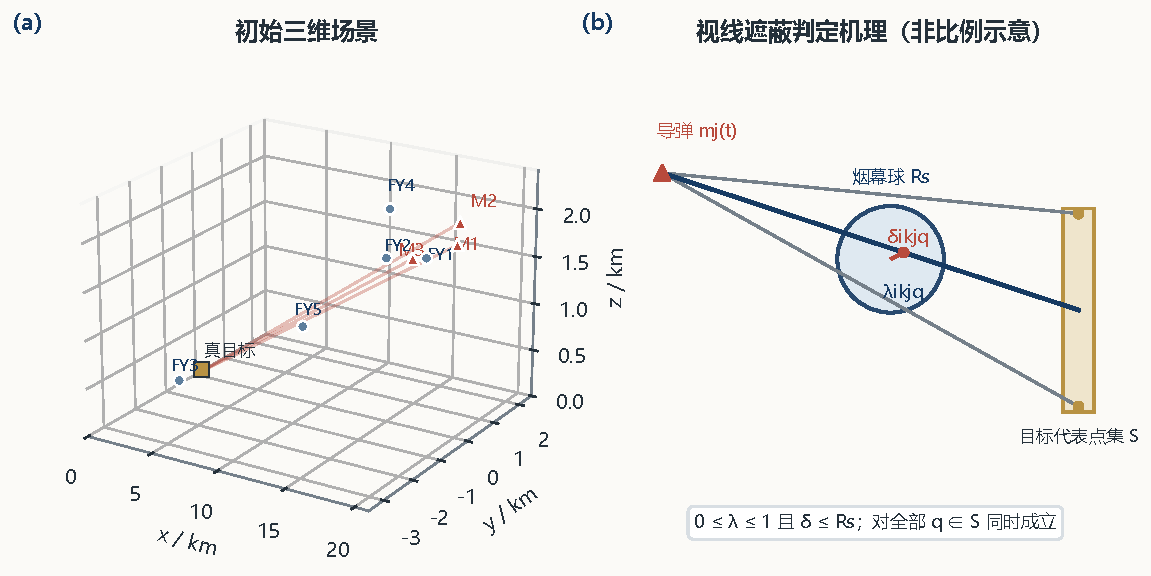
\includegraphics[width=0.98\linewidth]{PF002_scene_los.pdf}
\caption{初始空间与多视线遮蔽判据。左图按千米尺度给出三枚导弹、五架无人机与真目标的初始关系；右图说明烟幕中心对导弹—目标代表点视线的投影参数与垂距条件，右图不按物理比例。}
\label{fig:pf002}
\end{figure}

\subsection{分问策略}

Q1 只复算题面固定参数；Q2 将 FY1 的航向、速度、投放时刻和起爆延迟作为连续变量；Q3 在 Q2 基础上增加三弹时序和同机间隔；Q4 对三架无人机分别设置连续变量；Q5 进一步增加弹位使用与主目标指派，并采用总时长优先、最短时长次之的严格字典序目标。各问最终都归结为“生成单弹有效区间—按导弹求并集—计算目标值”。

\section{模型假设与符号}

\subsection{关键假设及风险}

表~\ref{tab:assumptions}列出对结果含义最关键的冻结假设。A03、A08 和 A11 会实质影响数值或任务分配，因此在第~\ref{sec:validation}节单独检验；空气阻力、风场等未建模因素作为外推边界保留。

\begin{table}[H]
\centering
\caption{关键冻结假设与验证方式}
\label{tab:assumptions}
\small
\begin{tabularx}{\textwidth}{cL c L}
\toprule
编号 & 假设 & 风险 & 验证或边界 \\
\midrule
A01--A02 & 导弹飞向原点；无人机一次转向后定高、定速、定航向 & 低 & 与题面坐标和速度约束逐项核对 \\
A03--A04 & 干扰弹继承无人机水平速度，初始竖直速度为 0；忽略阻力，\(g=9.8\) & 中 & 对“不继承水平速度”情景复算 \\
A05--A07 & 烟幕不起水平漂移，以 \(3\,\mathrm{m/s}\) 下沉；到地面停止计时 & 中 & 与“到地面后停留”口径比较 \\
A08 & 目标圆柱全部代表点同时被遮挡才有效 & 高 & 与中心点、固定格点和 \(80\%\) 覆盖比较 \\
A09 & 多弹遮蔽时长按时间区间并集统计 & 中 & 重叠、相邻和空区间单元测试 \\
A10--A12 & Q5 每枚已用弹登记一个主目标；总时长优先、最短时长次之；三导弹均须正遮蔽 & 高 & 指派唯一性与目标优先级敏感性 \\
\bottomrule
\end{tabularx}
\end{table}

\subsection{主要符号}

\begin{table}[H]
\centering
\caption{主要符号说明}
\label{tab:symbols}
\small
\begin{tabularx}{0.98\textwidth}{cL cL}
\toprule
符号 & 含义 & 符号 & 含义 \\
\midrule
\(i,j,k\) & 无人机、导弹与弹位编号 &
\(\vect m_{j0},\vect u_{i0}\) & 导弹、无人机初始位置 \\
\(\theta_i,v_i\) & 无人机航向角与速度 &
\(r_{ik},\tau_{ik},d_{ik}\) & 投放时刻、延迟与起爆时刻 \\
\(\vect b_{ik}(t)\) & 起爆前干扰弹位置 &
\(\vect c_{ik}(t)\) & 起爆后烟幕中心位置 \\
\(\lambda_{ikjq},\delta_{ikjq}\) & LOS 投影参数与垂距 &
\(\mathcal S\) & 真目标确定性代表点集 \\
\(\mathcal I_{ikj},D_{ikj}\) & 单弹有效区间与时长 &
\(\mathcal U_j,T_j\) & 导弹 \(j\) 的并集与总时长 \\
\(x_{ikj},y_{ik}\) & 主目标指派与弹位使用变量 &
\(\mu(\cdot)\) & 时间集合的测度 \\
\bottomrule
\end{tabularx}
\end{table}

\section{三维运动学与遮蔽模型}

模型的数据流和约束位置如图~\ref{fig:pf001}所示。该结构把物理运动、几何判定和优化目标分开：任何搜索器只能改变冻结的决策变量，不能改变烟幕半径、目标几何或有效遮蔽定义。

\begin{figure}[H]
\centering
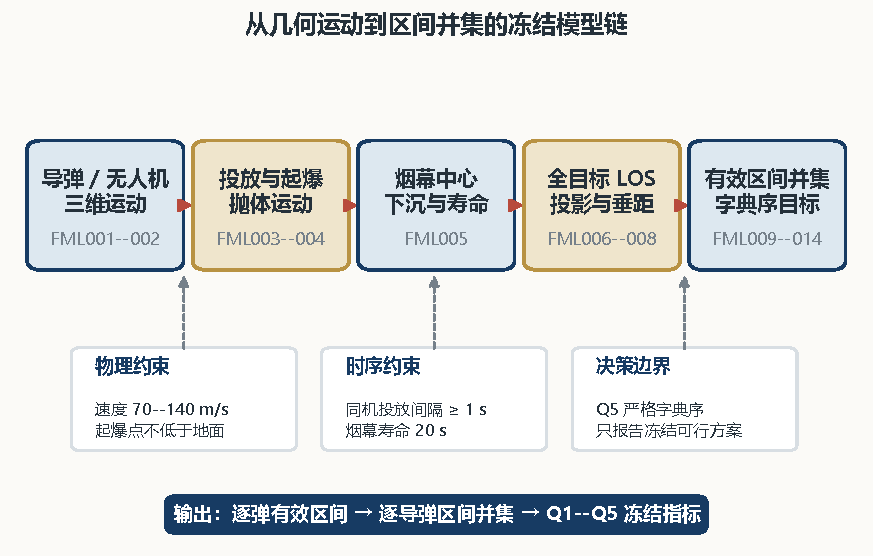
\includegraphics[width=0.98\linewidth]{PF001_model_chain.pdf}
\caption{冻结模型链与约束结构。五级主链对应公式 FML001--FML014；下方约束分别限制物理可行性、投放时序和 Q5 决策口径。}
\label{fig:pf001}
\end{figure}

\subsection{导弹、无人机与干扰弹轨迹}

导弹 \(j\) 始终指向假目标原点，其单位方向与轨迹为
\begin{equation}
\vect e_{Mj}=-\frac{\vect m_{j0}}{\lVert\vect m_{j0}\rVert},\qquad
\vect m_j(t)=\vect m_{j0}+v_M\vect e_{Mj}t,\qquad
t_j^{\mathrm{hit}}=\frac{\lVert\vect m_{j0}\rVert}{v_M}.
\label{eq:missile-trajectory}
\end{equation}
无人机在水平面内保持固定航向：
\begin{equation}
\vect e_i(\theta_i)=(\cos\theta_i,\sin\theta_i,0)^{\mathsf T},\qquad
\vect u_i(t)=\vect u_{i0}+v_i\vect e_i(\theta_i)t,
\quad 70\le v_i\le140.
\label{eq:uav-trajectory}
\end{equation}
第 \(k\) 枚干扰弹在 \(r_{ik}\) 时刻释放，并继承无人机水平速度。对
\(r_{ik}\le t\le d_{ik}\)，有
\begin{equation}
\vect b_{ik}(t)=\vect u_{i0}+v_i\vect e_i(\theta_i)t
-\frac12 g(t-r_{ik})^2\vect e_z .
\label{eq:bomb-trajectory}
\end{equation}
令 \(d_{ik}=r_{ik}+\tau_{ik}\)，起爆点和延迟约束为
\begin{equation}
\vect p_{ik}^{\mathrm{det}}
=\vect u_{i0}+v_i\vect e_i(\theta_i)d_{ik}
-\frac12g\tau_{ik}^{2}\vect e_z,\qquad
0\le\tau_{ik}\le\sqrt{\frac{2z_{i0}}{g}}.
\label{eq:detonation}
\end{equation}
烟幕形成后仅竖直下沉，其有效终点同时受 \(20\,\mathrm s\) 寿命与地面约束：
\begin{equation}
\vect c_{ik}(t)=\vect p_{ik}^{\mathrm{det}}-w_s(t-d_{ik})\vect e_z,\qquad
t_{ik}^{\mathrm{end}}=
\min\!\left(d_{ik}+T_s,\ d_{ik}+\frac{z_{ik}^{\mathrm{det}}}{w_s}\right).
\label{eq:smoke-trajectory}
\end{equation}

\subsection{圆柱目标与多视线遮挡}

真目标圆柱及其代表点集写为
\begin{equation}
\mathcal C_T=\{(x,y,z):x^2+(y-200)^2\le R_T^2,\ 0\le z\le H_T\},
\qquad
\mathcal S=\mathcal S_{\mathrm{side}}\cup\mathcal S_{\mathrm{top}}\cup\mathcal S_{\mathrm{bottom}}.
\label{eq:target-cylinder}
\end{equation}
对代表点 \(\vect q\in\mathcal S\)，从导弹位置到目标点的线段为
\(\vect m_j(t)+\lambda[\vect q-\vect m_j(t)]\)。烟幕中心在该直线上的投影参数和垂距为
\begin{equation}
\lambda_{ikjq}(t)=
\frac{[\vect c_{ik}(t)-\vect m_j(t)]^{\mathsf T}[\vect q-\vect m_j(t)]}
{\lVert\vect q-\vect m_j(t)\rVert^2},
\quad
\delta_{ikjq}(t)=
\left\|\vect c_{ik}(t)-\vect m_j(t)-\lambda_{ikjq}(t)[\vect q-\vect m_j(t)]\right\|.
\label{eq:los-clearance}
\end{equation}
只有投影落在线段上且垂距不超过烟幕半径，才遮挡该代表点；全部代表点同时满足时，单弹有效指示量为
\begin{equation}
\chi_{ikj}(t)=
\prod_{\vect q\in\mathcal S}
\mathbf 1\!\left[0\le\lambda_{ikjq}(t)\le1\ \land\ \delta_{ikjq}(t)\le R_s\right].
\label{eq:occlusion-indicator}
\end{equation}
该全点口径比只检查目标中心更保守，避免把仅遮住圆柱局部的烟幕误计为完全有效。

\subsection{连续时间区间与目标函数}

单弹对导弹 \(j\) 的有效时间集合及其时长为
\begin{equation}
\mathcal I_{ikj}=
\left\{t\in\left[d_{ik},\min(t_{ik}^{\mathrm{end}},t_j^{\mathrm{hit}})\right]:
\chi_{ikj}(t)=1\right\},
\qquad D_{ikj}=\mu(\mathcal I_{ikj}).
\label{eq:single-bomb-interval}
\end{equation}
对于已使用弹位 \(y_{ik}=1\)，同一导弹的总有效区间和时长为
\begin{equation}
\mathcal U_j=\bigcup_{i,k:\,y_{ik}=1}\mathcal I_{ikj},
\qquad T_j=\mu(\mathcal U_j).
\label{eq:interval-union}
\end{equation}
区间并集保证重叠部分只计一次。Q2 最大化单弹时长；Q3--Q4 最大化 M1 的区间并集，并加入同机投放间隔：
\begin{equation}
\max D_{\mathrm{FY1},1,\mathrm{M1}},\qquad
\max T_{\mathrm{M1}},\qquad
r_{i,k+1}-r_{ik}\ge1\ \mathrm s.
\label{eq:q234-objective}
\end{equation}
Q5 采用严格字典序目标
\begin{equation}
\operatorname*{lex\,max}_{\vect x,\vect y,\Theta,V,R,\Tau}
\left(\sum_{j\in\{\mathrm{M1,M2,M3}\}}T_j,\ 
\min_{j\in\{\mathrm{M1,M2,M3}\}}T_j\right),
\label{eq:q5-objective}
\end{equation}
并满足
\begin{equation}
x_{ikj},y_{ik}\in\{0,1\},\qquad
\sum_{j\in\mathcal M}x_{ikj}=y_{ik},\qquad
\sum_{i,k}x_{ikj}\mathbf 1[D_{ikj}>0]\ge1,\quad \forall j\in\mathcal M.
\label{eq:q5-assignment}
\end{equation}
二级目标仅用于一级目标值相同的方案比较，不引入未登记的近似最优容差。

\section{求解方法与复现设置}

\subsection{混合求解流程}

有效时长由布尔几何判定与区间边界共同决定，目标函数非光滑且无显式梯度。Q2--Q4 先用差分进化进行连续空间候选搜索，再以 Powell 无导数方法精修；两类算法的方法来源分别见文献~\cite{storn1997de,powell1964efficient}。Q5 外层筛选满足正覆盖约束的离散指派，内层复用连续求解器，最后按严格字典序比较目标二元组。

一次方案评价依次执行：生成运动轨迹；在烟幕有效窗口扫描 \(\chi_{ikj}(t)\)；对真假切换点二分求根；合并重叠/相邻区间；检查速度、起爆高度、投放间隔和指派约束；输出逐弹区间及逐导弹并集。Q1 不参与优化，只用于检验整条评价链。

\begin{table}[H]
\centering
\caption{搜索与最终严格复算设置}
\label{tab:numerical-config}
\small
\begin{tabularx}{0.98\textwidth}{lY lY}
\toprule
项目 & 设置 & 项目 & 设置 \\
\midrule
候选全局搜索 & 差分进化 &
局部精修 & Powell 无导数法 \\
加密搜索代表点 & \(16\times4\times3\) &
最终严格复算代表点 & \(20\times5\times4\) \\
加密扫描步长 & \(0.05\,\mathrm s\) &
严格扫描步长 & \(0.025\,\mathrm s\) \\
加密求根容差 & \(10^{-6}\,\mathrm s\) &
严格求根容差 & \(10^{-7}\,\mathrm s\) \\
加密搜索规模 & \(\mathrm{maxiter}=12,\ \mathrm{popsize}=8\) &
稳定性种子 & 20250722、20250723、20250724 \\
冻结包 & RF-20260722T114756Z &
结果边界 & 冻结可行方案，不证明全局最优 \\
\bottomrule
\end{tabularx}
\end{table}

\section{五问结果与解释}

\subsection{Q1 固定方案与 Q2 单弹优化}

Q1 的投放时刻为 \(1.5\,\mathrm s\)，起爆延迟为 \(3.6\,\mathrm s\)，故起爆时刻为 \(5.1\,\mathrm s\)。严格复算得到有效区间
\([8.056308985,9.418510485]\,\mathrm s\)。Q2 冻结方案的有效区间更早开始且更晚结束，参数与结果见表~\ref{tab:q12-results}。

\begin{table}[H]
\centering
\caption{Q1--Q2 冻结参数与结果}
\label{tab:q12-results}
\scriptsize
\begin{tabular}{c c r r r r c r}
\toprule
问题 & 无人机/导弹 & 航向/\(^{\circ}\) & 速度/(\(\mathrm{m/s}\)) &
\(r\)/s & \(\tau\)/s & 有效区间/s & 时长/s \\
\midrule
Q1 & FY1/M1 & 180.000000 & 120.000000 & 1.500000 & 3.600000 &
\([8.056309,9.418510]\) & 1.362201500 \\
Q2 & FY1/M1 & 179.436545 & 130.083368 & 2.838973 & 4.978183 &
\([7.817156,10.055320]\) & 2.238164377 \\
\bottomrule
\end{tabular}
\end{table}

图~\ref{fig:pf003}把区间位置与精确时长分开表达。Q2 相对 Q1 增加
\(0.875962877\,\mathrm s\)，相对增幅 \(64.3049\%\)。这一结论仅比较题面固定策略与冻结搜索方案，不等价于理论全局最优性。

\begin{figure}[H]
\centering
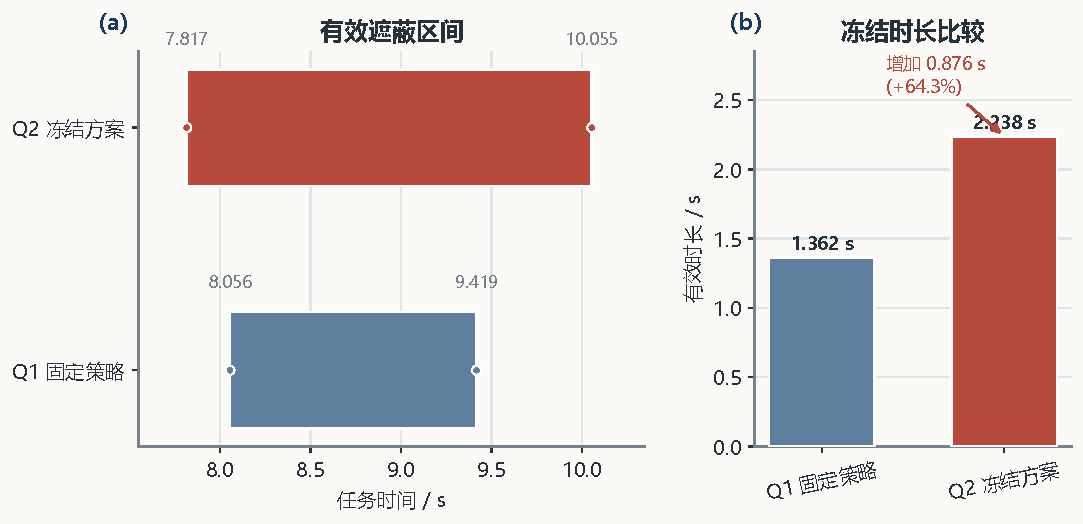
\includegraphics[width=0.96\linewidth]{PF003_q1_q2_comparison.pdf}
\caption{Q1 与 Q2 冻结区间及时长比较。Q2 的有效区间覆盖更长时间窗，对 M1 的时长较 Q1 增加 \(0.875962877\,\mathrm s\)。}
\label{fig:pf003}
\end{figure}

\subsection{Q3 同机三弹与 Q4 三机各一弹}

Q3 三枚弹使用同一航向与速度，相邻投放时刻恰好间隔 \(1\,\mathrm s\)，满足硬约束；Q4 分别评估 FY1--FY3。表~\ref{tab:q34-results}保留所有零贡献记录，而不是只展示并集值。

\begin{table}[H]
\centering
\caption{Q3--Q4 逐项贡献与并集结果}
\label{tab:q34-results}
\small
\begin{tabular}{c c c r r r c}
\toprule
问题 & 对象 & 弹号 & \(r\)/s & \(\tau\)/s & 单项时长/s & M1 并集/s \\
\midrule
\multirow{3}{*}{Q3}
& FY1 & 1 & 2.838973 & 4.978183 & 2.238164377 & \multirow{3}{*}{2.238164377} \\
& FY1 & 2 & 3.838973 & 4.978183 & 0 & \\
& FY1 & 3 & 4.838973 & 4.978183 & 0 & \\
\midrule
\multirow{3}{*}{Q4}
& FY1 & 1 & 2.838973 & 4.978183 & 2.238164377 & \multirow{3}{*}{2.238164377} \\
& FY2 & 1 & 1.500000 & 3.600000 & 0 & \\
& FY3 & 1 & 1.500000 & 3.600000 & 0 & \\
\bottomrule
\end{tabular}
\end{table}

\begin{figure}[H]
\centering
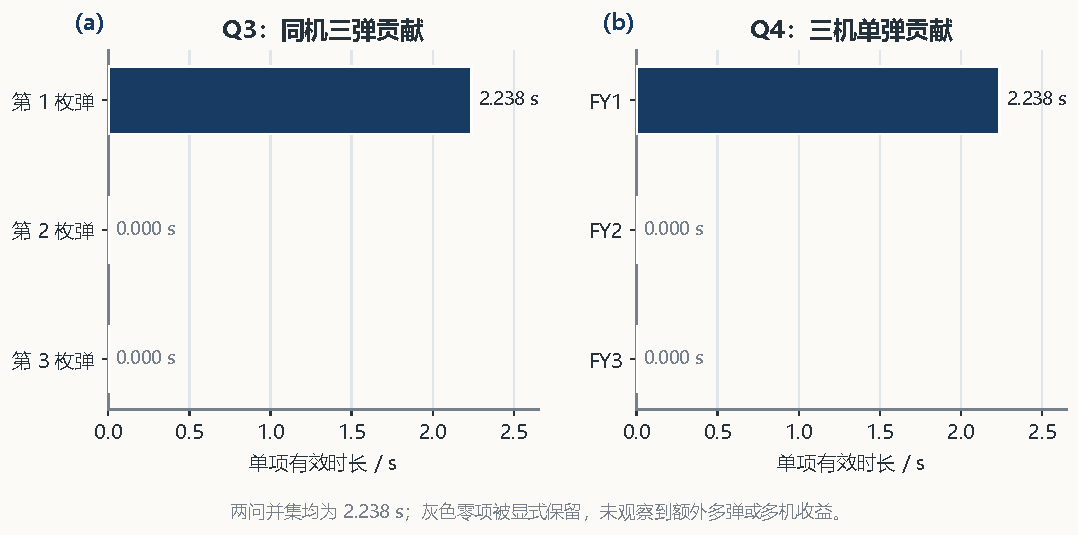
\includegraphics[width=0.96\linewidth]{PF004_q3_q4_contribution.pdf}
\caption{Q3 三弹与 Q4 三机的冻结贡献分解。两问只有 FY1 的第 1 枚弹形成有效区间，其余项为 \(0\)，故并集均未超过 Q2。}
\label{fig:pf004}
\end{figure}

零贡献说明在当前全点判据、冻结搜索预算与可达几何下，额外资源没有形成新增有效区间；它不证明所有可能策略都不存在协同收益。该边界避免把“资源投入”直接等同于“有效遮蔽增加”。

\subsection{Q5 五机多弹多目标分配}

Q5 的冻结方案只启用三个弹位：FY1-B1 指向 M1，FY2-B1 指向 M2，FY5-B1 指向 M3；FY3、FY4 与其余弹位保持未使用。指派关系见图~\ref{fig:pf005}，连续参数见表~\ref{tab:q5-results}。

\begin{figure}[H]
\centering
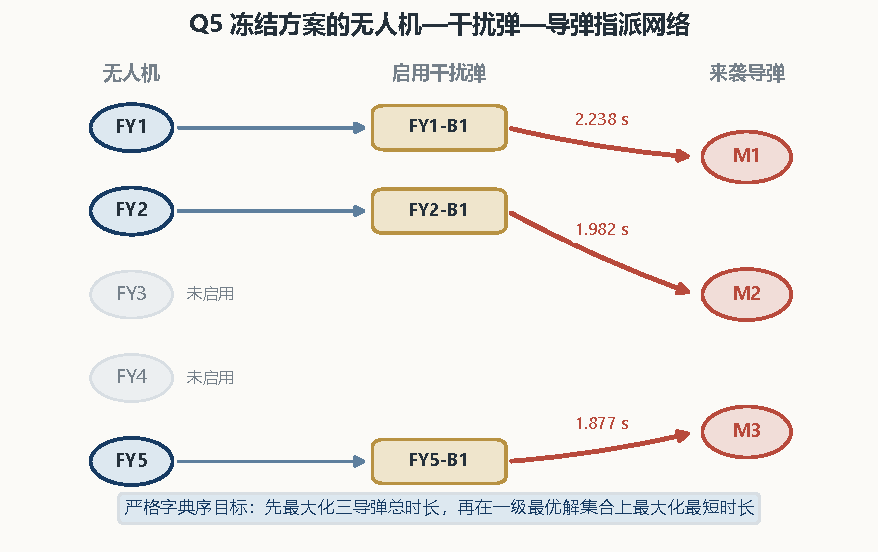
\includegraphics[width=0.96\linewidth]{PF005_q5_assignment.pdf}
\caption{Q5 冻结指派网络。三条红色边分别绑定 FY1-B1、FY2-B1、FY5-B1 与 M1、M2、M3；灰色节点表示未启用无人机，不产生正式目标贡献。}
\label{fig:pf005}
\end{figure}

\begin{table}[H]
\centering
\caption{Q5 启用弹位的冻结策略}
\label{tab:q5-results}
\scriptsize
\resizebox{\textwidth}{!}{
\begin{tabular}{c c r r r r c c r}
\toprule
无人机 & 目标 & 航向/\(^{\circ}\) & 速度/(\(\mathrm{m/s}\)) &
\(r\)/s & \(\tau\)/s & 起爆点 \((x,y,z)\)/m & 有效区间/s & 时长/s \\
\midrule
FY1 & M1 & 179.436545 & 130.083368 & 2.838973 & 4.978183 &
\((16783.167,10.000,1678.567)\) & \([7.817156,10.055320]\) & 2.238164377 \\
FY2 & M2 & 275.597098 & 100.886906 & 6.085791 & 3.555641 &
\((12094.869,431.943,1338.051)\) & \([9.641432,11.623475]\) & 1.982043314 \\
FY5 & M3 & 119.302179 & 121.141313 & 13.136138 & 2.169562 &
\((12092.549,-383.085,1276.936)\) & \([15.305700,17.182501]\) & 1.876800871 \\
\bottomrule
\end{tabular}}
\end{table}

由三个区间分别求得
\[
(T_{\mathrm{M1}},T_{\mathrm{M2}},T_{\mathrm{M3}})
=(2.238164377,\ 1.982043314,\ 1.876800871)\ \mathrm s.
\]
因此一级目标为 \(6.097008562\,\mathrm s\)，二级目标为
\(1.876800871\,\mathrm s\)。图~\ref{fig:pf006}同时展示区间在任务时间轴上的位置与字典序目标摘要。

\begin{figure}[H]
\centering
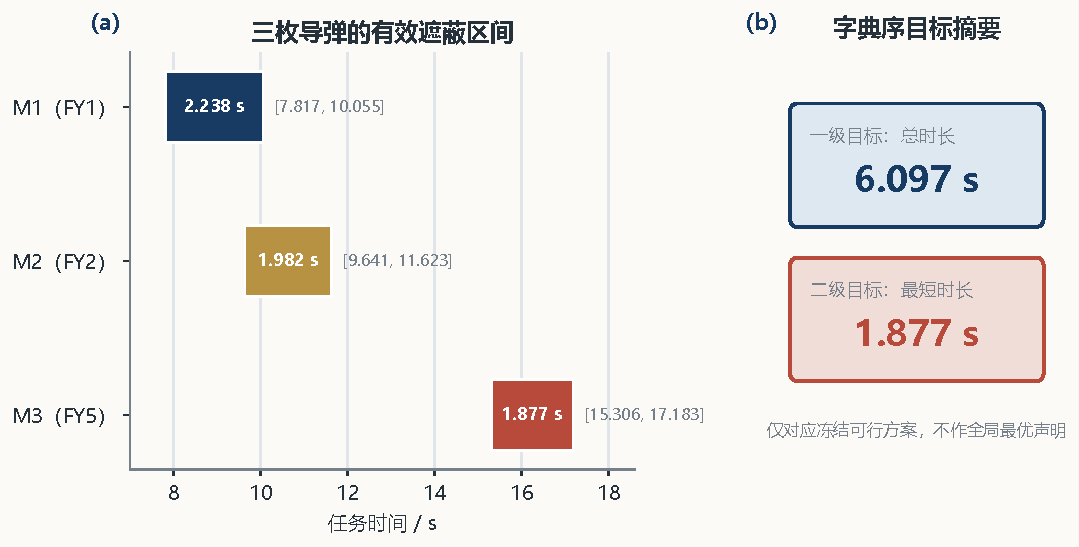
\includegraphics[width=0.96\linewidth]{PF006_q5_intervals.pdf}
\caption{Q5 三枚导弹的冻结有效区间与目标摘要。区间起点反映各自起爆和几何时窗；总时长与最短时长分别对应严格字典序的一级、二级目标。}
\label{fig:pf006}
\end{figure}

\section{数值验证、敏感性与边界}
\label{sec:validation}

\subsection{一致性、约束与稳定性}

独立复核首先从逐弹区间端点重新计算每条记录的长度，再按导弹合并区间，所得九项汇总指标与冻结 CSV、结果合同逐项一致，最大绝对差为 \(0\)。全部启用计划满足速度、非负时序、起爆高度、Q3 投放间隔与 Q5 正覆盖约束；Q5 的三条主目标指派互异且均产生正时长。

三个登记随机种子在相同配置下逐指标跨度为 \(0\)。最终严格复算相对上一档加密配置的最大绝对变化为 \(2.039\times10^{-4}\,\mathrm s\)，出现在 Q1，约占 Q1 冻结值的 \(0.015\%\)；其余核心指标差异处于微秒量级。图~\ref{fig:pf007}只说明已登记分辨率、预算与种子范围内的数值稳定性，不构成搜索空间全局收敛证明。

\begin{figure}[H]
\centering
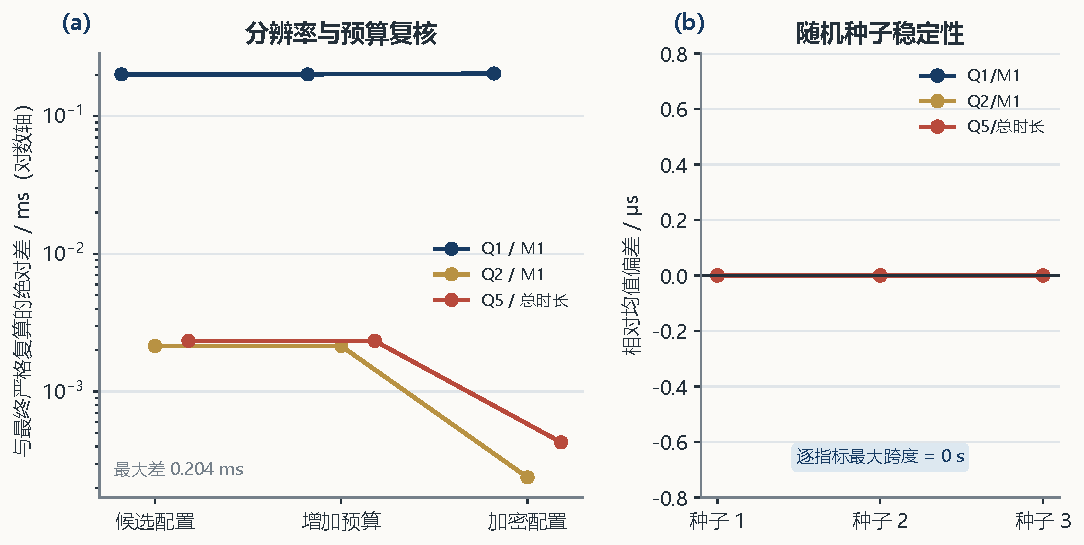
\includegraphics[width=0.96\linewidth]{PF007_convergence_stability.pdf}
\caption{数值分辨率、预算与随机种子复核。左图为候选、增预算和加密配置相对最终严格复算的绝对差；右图显示三个随机种子的逐指标偏差均为 \(0\)。}
\label{fig:pf007}
\end{figure}

\subsection{基线与高风险假设}

\begin{table}[H]
\centering
\caption{冻结结果的验证与敏感性摘要}
\label{tab:validation}
\small
\begin{tabularx}{\textwidth}{l r L}
\toprule
检验 & 最大变化 & 解释边界 \\
\midrule
三随机种子 & \(0\,\mathrm s\) & 相同配置下逐指标完全一致 \\
严格复算对上一档加密 & \(2.039\times10^{-4}\,\mathrm s\) & 数值分辨率差异，不改变正文结论 \\
中心点基线 & \(0.449\,\mathrm s\) & 只遮挡目标中心会放宽主模型 \\
固定格点基线 & \(0.123\,\mathrm s\) & 离散格点用于口径对照，不替代连续边界 \\
A03 无水平继承 & \(2.238\,\mathrm s\) & 当前各项均降至 \(0\)，高度敏感 \\
A07 地面停留 & \(0\,\mathrm s\) & 当前有效区间早于触地，结果不变 \\
A08 \(80\%\) 覆盖 & \(0.232401\,\mathrm s\) & M2 增量最大，遮挡定义影响评价 \\
A11 公平优先 & 指派改变 & 总时长降至 \(6.080232\,\mathrm s\)，最短时长升至 \(1.908269\,\mathrm s\) \\
\bottomrule
\end{tabularx}
\end{table}

图~\ref{fig:pf008}把五种几何/物理情景相对冻结全点模型的变化统一到同一尺度。A03 取消水平速度继承后，当前投放点与起爆点的可达关系被根本改变，所有登记时长降为 \(0\)；A07 不变是因为现有有效区间内烟幕尚未触地，不能外推为“地面边界永远不重要”；A08 放宽遮挡比例后各指标不下降，且 M2 增加 \(0.232401085\,\mathrm s\)，说明全点口径具有实质保守性。

\begin{figure}[H]
\centering
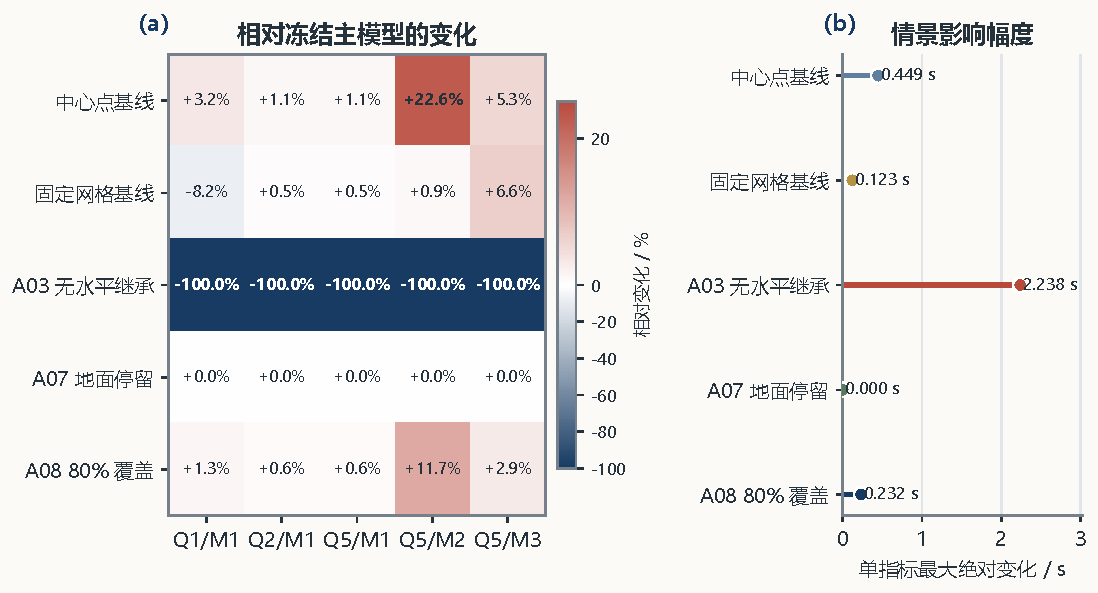
\includegraphics[width=0.97\linewidth]{PF008_sensitivity.pdf}
\caption{主模型基线与假设敏感性。热力图给出各指标相对冻结全点模型的百分比变化，右图给出单指标最大绝对变化；A03 与 A08 是当前结果的主要口径风险。}
\label{fig:pf008}
\end{figure}

\section{模型评价与改进方向}

\subsection{模型优点}

模型具有五点优势：运动轨迹、起爆点、烟幕中心和导弹视线均可复算，\textbf{物理链可解释}；保留圆柱目标并采用全点判据，\textbf{几何口径保守}；连续边界求根与区间并集避免重叠时间重复累计，\textbf{多弹计量严谨}；同一评价器覆盖 Q1 固定计算、Q2--Q4 连续优化和 Q5 混合决策，\textbf{结构统一}；零贡献、种子、加密复算和高风险假设均如实保留，\textbf{证据边界明确}。

\subsection{局限与可扩展方向}

模型忽略空气阻力、风场与烟幕扩散形变；若获得气象参数，应把 \(\vect c_{ik}(t)\) 扩展为含风漂移与扩散半径的随机过程，并报告置信区间。圆柱代表点法仍是离散近似；若进一步加密不稳定，可改用导弹视点下圆柱投影轮廓与烟幕球投影的解析包含判据。Q3、Q4 的零新增贡献可能来自严格全点口径、可达性或有限搜索结构，后续应增加专门的区间互补初始化，而不能直接宣称多弹/多机无效。Q5 对目标优先级敏感，实际决策前应由任务方确认总效能与公平性的权重。

\section{结论}

统一的三维运动学、多视线判据和区间并集框架可覆盖五个递进子问题。Q2 将 Q1 的 M1 时长由 \(1.362201500\,\mathrm s\) 提高到 \(2.238164377\,\mathrm s\)；Q3、Q4 的额外资源没有形成新增区间。Q5 由 FY1、FY2、FY5 分别服务 M1、M2、M3，总时长为 \(6.097008562\,\mathrm s\)，最短时长为 \(1.876800871\,\mathrm s\)。复核检查均通过；结果对 A03、A08 敏感，对当前方案中的 A07 不敏感。上述结论不构成全局最优证明。

\bibliographystyle{unsrt}
\bibliography{final_references}

\end{document}
